
\documentclass{article}

\usepackage{amsmath}
\usepackage{comment}
\usepackage{amscd}
\usepackage[tableposition=top]{caption}
\usepackage{ifthen}
\usepackage[utf8]{inputenc}

\usepackage{Sweave}
\begin{document}

\title{A DualBrothers Demo}
\author{Jan Irvahn}
\maketitle

This is a demo for using the java program, DualBrothers, in R.  To
get started, install the dualbrothers R package from the directory that contains the dualbrothers\_0.0-1.tar.gz file. The rJava packages will need to be installed. On a linux machine you can use the following commands.
\begin{verbatim}
R CMD INSTALL rbrothers
\end{verbatim}
Copy the extdata directory from the default R installation folder to your current location and change your directory into the KAL153 folder.
\begin{verbatim}
cp <path-to-R-packages>/rbrothers/extdata .
cd extdata/KAL153/					    
\end{verbatim}

Start R and load the dualbrothers library.

\begin{Schunk}
\begin{Sinput}
> library(rbrothers)
\end{Sinput}
\end{Schunk}

Now you can run dualbrothers with a single command.
\begin{Schunk}
\begin{Sinput}
> x<-dualbrothers(123, "KAL153", format = "interleaved")
\end{Sinput}
\end{Schunk}

Plots can be created with the following commands.
\begin{Schunk}
\begin{Sinput}
> plot(x)
> plottree.db(x)
\end{Sinput}
\end{Schunk}

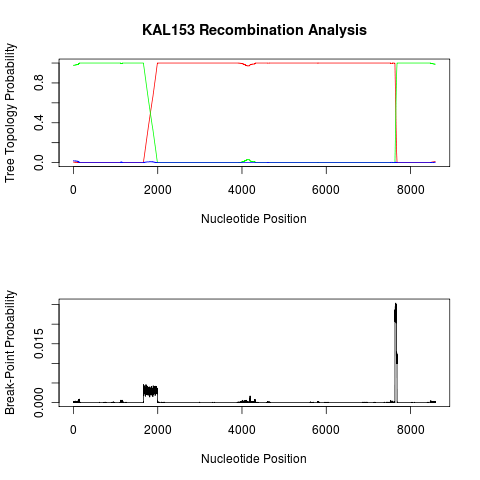
\includegraphics[width=70mm]{KAL153p1.png}
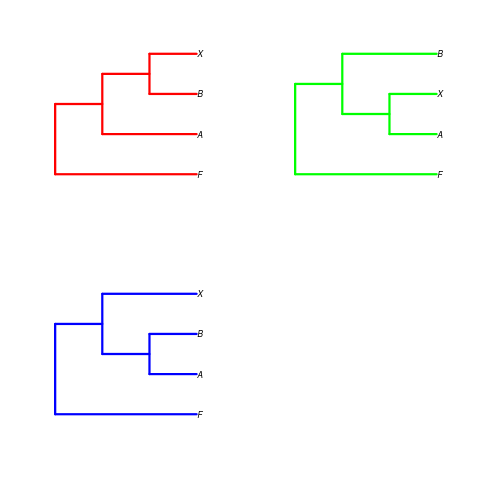
\includegraphics[width=70mm]{KAL153p2.png}

\end{document}

